\section{Spracovávané Dáta}

Budeme spracovávať štatistické dáta pacientov, ktorý užívali dva rôzne lieky (nikdy nie naraz) proti primárnej chorobe. Máme k dispozícii dáta o vzorke 10~000 pacietov.


K dispozícii máme, aký liek bol podávaný pacientovi a aký účinok to malo na jeho primárne ochorenie. Ďalej máme k dispozícii základné fyzické proporcie pacienta ako: vek, index telesnej hmotnosti a priemerný krvný tlak. Je nám známa taktiež anamnéza pacienta (výskyt sekundárnych chorôb pred a po liečbe a iná nešpecifikovaná medikácia).

\subsection{Vekové spektrum}

Máme k dispozícii dáta pacientov so širokým vekovým spektrom, ktoré môžme vidieť v histograme~\ref{fig:hist-vek}. Histogram udáva absolútny počet pacientov v jednotlivých vekových kategóriach. Pomocou t-testu sme si overili normálne rozdelenie týchto veličín na hladine štatistickej významnosti (0.05). V tabuľke~\ref{tab:vek} je rozdelenie pacientov do vekových podskupín.

\begin{figure}[h!]
	\centering
  		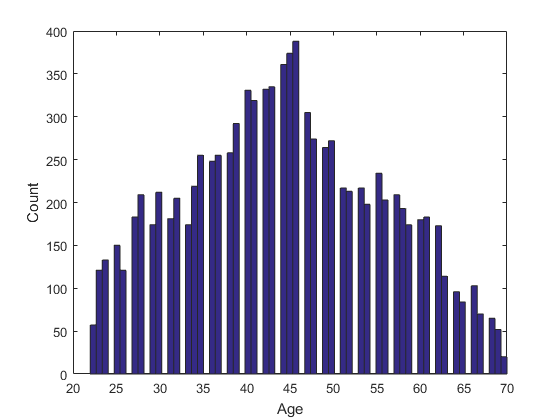
\includegraphics[width=0.9\textwidth]{ages.png}
  	\caption{Histogram Vekov}
  	\label{fig:hist-vek}
\end{figure}

\begin{table}[h!]
\centering
\begin{tabular}{c|ccccc}
\hline
\textbf{Vek}             & \textless 30 & 30-39 & 40-49 & 50-59 & 60\textless \\ \hline
\textbf{Počet Pacientov} & 1148 & 2299  & 3283  & 2130  & 1140 \\ \hline
\end{tabular}
\caption{Vek pacientov}
\label{tab:vek}
\end{table}

\subsection{BMI spektrum}

BMI (ang. Body Mass Index) je index telesnej hmotnosti. Je to pomer medzi aktuálnou váhou a výškou\textsuperscript 2. V histograme~\ref{fig:hist-bmi} je rozloženie BMI pacientov. V tabuľke~\ref{tab:vek} sú dáta zobrazené v jednotlivých podskupinách. Za pomoci t-testom sme si overili normálne rozdelenie veličín na hladine štatistickej významnosti (0.05).

\begin{figure}[h!]
	\centering
  		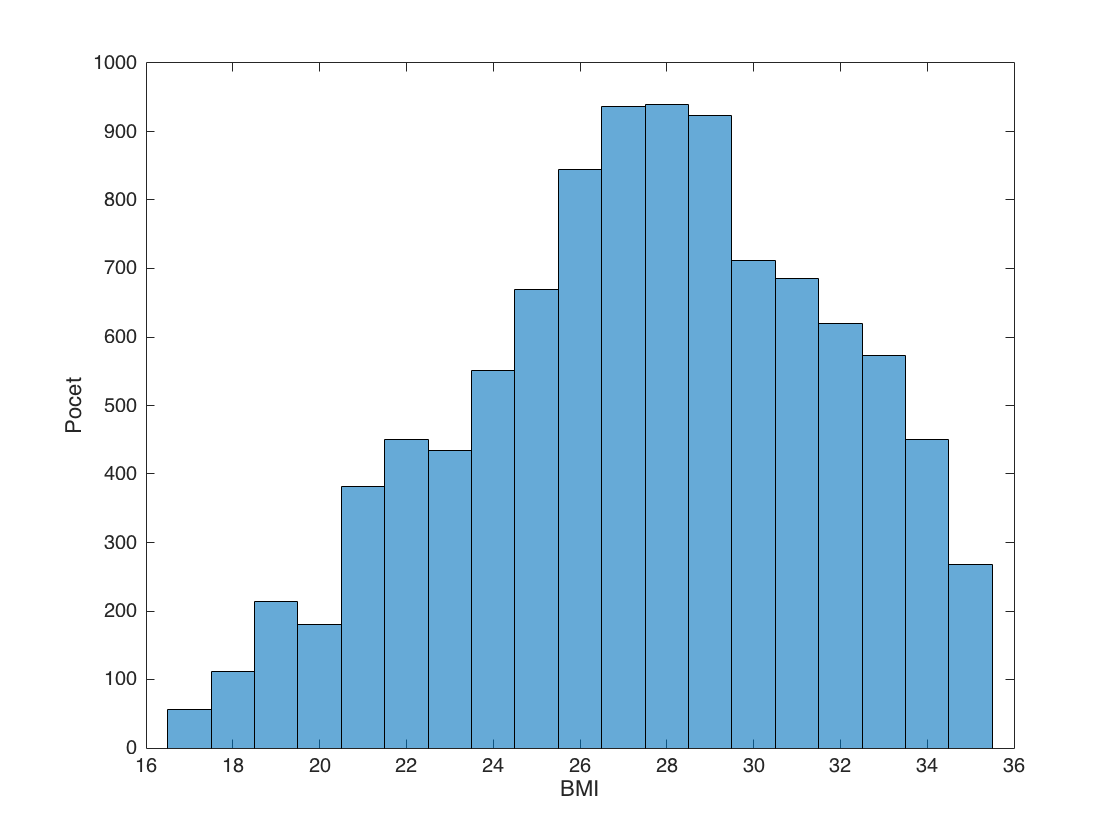
\includegraphics[width=0.9\textwidth]{histBmi.png}
  	\caption{Histogram BMI}
  	\label{fig:hist-bmi}
\end{figure}

\begin{table}[h!]
\centering
\begin{tabular}{c|cccc}
\hline
\textbf{BMI} & Podvýživa & Zdravá Váha & Mierna Nadváha & Obezita \\ \hline
\textbf{Počet Pacientov} & 167       & 2212        & 4314           & 3307    \\ \hline
\end{tabular}
\caption{BMI Pacientov}
\label{tab:bmi}
\end{table}






\subsection{MAP spektrum}

MAP (ang. Mean Arterial Pressure) je priemerný krvný tlak udávaný v mmHg. Rozdelenie medzi pacientami môžme vidieť v histograme \ref{fig:histMAP} a rozdelenie do podskupín v tabuľke \ref{tab:map}.

\begin{figure}[h!]
	\centering
  		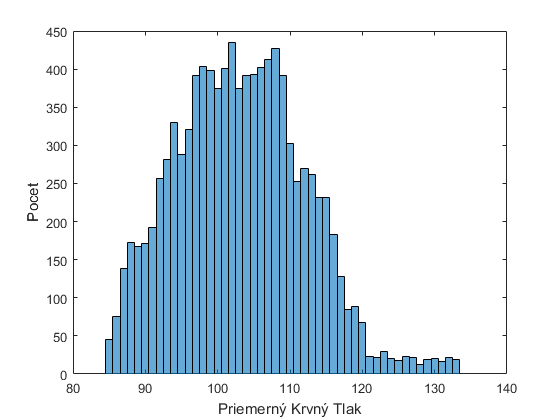
\includegraphics[width=0.9\textwidth]{pressures.png}
  	\caption{Histogram MAP}
  	\label{fig:histMAP}
\end{figure}


\begin{table}[h!]
\centering
\begin{tabular}{c|ccccc}
\hline
\textbf{MAP} & \textless70 & 70-92 & 93-105 & 106-119 & 120\textless \\ \hline
\textbf{Počet Pacientov} & 0 & 1218  & 4785   & 3665 & 332 \\ \hline
\end{tabular}
\caption{MAP Pacientov}
\label{tab:map}
\end{table}


\subsection{Lieky a Medikácia}

V tabuľke \ref{tab:sick-healthy} môžme vidieť počet vyliečených a nevyliečených pacientov (primárna choroba) po podaní lieku 1 a lieku 2. 

\begin{table}[h!]
\centering
\begin{tabular}{l|lll}
\hline
                     & \textbf{Liek 1} & \textbf{Liek 2} & \textbf{Celkom} \\ \hline
\textbf{Vyliečený}   & 1625            & 3630            & 5255            \\ \hline
\textbf{Nevyliečený} & 3837            & 908             & 4745            \\ \hline
\textbf{Celkom}      & 5462            & 4538            & 10 000          \\ \hline
\end{tabular}
\caption{Vyliečený a nevyliečený pacienti s rôznými liekmi}
\label{tab:sick-healthy}
\end{table}

V tabuľke \ref{tab:ucinnost} vidíme účinnosť jednotlivých liekov na našej vzorke. Účinnosť myslíme ako pomer vyliečených k celkovému počtu pacientov liečených danným liekom.

\begin{table}[h!]
\centering
\begin{tabular}{l|ll}
\hline
                  & \textbf{Liek 1} & \textbf{Liek 2} \\ \hline
\textbf{Účinnosť} & 29,75\%         & 80\%            \\ \hline
\end{tabular}
\caption{Účinnosť jednotlivých liekov}
\label{tab:ucinnost}
\end{table}

V tabuľke \ref{tab:sekundarne} pozorujeme pridružené sekundárne choroby pred a po liečbe daným typom lieku.

\begin{table}[h!]
\centering
\begin{tabular}{c|cc}
\hline
                             & \textbf{1. sek. choroba} & \textbf{2. sek. choroba} \\ \hline
\textbf{Výskyt pred liečbou} & 4717                             & 6387                              \\ \hline
\textbf{Výskyt po liečbe}    & 4505                             & 3888                              \\ \hline
\end{tabular}
\caption{Výskyt sekundárnych chorôb pred a po liečbe}
\label{tab:sekundarne}
\end{table}





























